\documentclass[12pt,a4paper]{article}
\usepackage{cmap}
\usepackage{amsmath}
\usepackage{amsfonts}
\usepackage{mathtext}
\usepackage{titlesec}
\usepackage{float}
\usepackage{subcaption}
\usepackage{amssymb}
\usepackage[utf8]{inputenc}
\usepackage[T2A]{fontenc}
\usepackage{wrapfig}
\usepackage[english, russian]{babel}
\usepackage[left=2cm,right=2cm,top=2cm,bottom=2cm]{geometry}
\usepackage{indentfirst}

\DeclareSymbolFont{T2Aletters}{T2A}{cmr}{m}{it}

%%% Работа с картинками
\usepackage{graphicx}  % Для вставки рисунков
\graphicspath{{imgs/}}  % папки с картинками

\usepackage{caption}
\captionsetup{labelsep=period, labelfont=bf}

\titleformat{\section}[block]
{\normalfont}{\thesection.}{0 cm}{}
\titleformat{\subsection}[block]
{\bfseries}{\thesubsection.}{0 cm}{}

\titlespacing{\section}{17pt}{14pt}{10pt}
\titlespacing{\subsection}{17pt}{14pt}{4pt}

\def \TITLE {Отчет о выполнении лабораторной работы №3.7.1}
\def \SUBTITLE {Скин-эффект в полом цилиндре}
\def \AUTHOR {Выполнил студент группы Б03-405\\ Тимохин Даниил}
\def \DATE {24 октября 2025 г.}

\begin{document}

\begin{titlepage}
	\centering
	\vspace{5cm}
	{\scshape\large Московский физико-технический институт \\
	(НАЦИОНАЛЬНЫЙ ИССЛЕДОВАТЕЛЬСКИЙ УНИВЕРСИТЕТ)}
	
	\vspace{4cm}
	{\LARGE \TITLE}
	
	\vspace{1cm}
	{\Huge\bf \SUBTITLE }
	
	\vspace{1cm}
	\vfill
	
\begin{flushright}
	{\LARGE \AUTHOR}
\end{flushright}
	

	\vfill

	\DATE
\end{titlepage}

\newpage

\fontsize{12}{14}\selectfont

\section{ Аннотация}
В данной работе исследуется скин-эффект в полом цилиндре. А также выполнение теории и нахождение проводимости самого цилиндра.


\section{ Теоретическая справка}

\begin{wrapfigure}{r}{0.5\textwidth}
    \includegraphics[width=0.5\textwidth]{ust.png}
    \caption{установка}
\end{wrapfigure}

Из уравнений максвелла следует, что
\begin{equation}
    \nabla^2 H=\sigma\mu\mu_0\frac{dH}{dt}
\end{equation}
Но из-за того, что мы используем медь, то можно считать $\mu=1$

Тогда если создать электро-магнитное поле катушкой:

$E=E(r) e^{iwt}$ и $H=H(r) e^{iwt}$

Также используя $E(r)=-\frac{1}{2}\mu_0 r\cdot iwH_0$ исходя цилиндрической симметрии задачи и связи электрического поля и магнитного. Получаем, что поле внутри и снаружи стенки должно быть одинаково, а значит можно брать за граничные условия напряженность поля в молиноидах, которые мы используем. С учетом граничных условий $H(0)=H_0$ и $H(h)=H_1$.

Ищем решение в виде $H(r)=Ae^(\alpha x)+Be^(-\alpha x)$ и тогда получим,
так как $\alpha=\sqrt{i\sigma\mu\omega}=\frac{1+i}{\delta}$, то
\begin{equation}
    \delta=\sqrt{\frac{2}{\sigma w\mu}}
\end{equation}

\begin{equation}
    H_1=\frac{H_0}{ch(\alpha h) +\frac{1}{2}a\alpha sh(\alpha h)}
\end{equation}

Подставляя глубину проникновения получаем при малых частотах получаем
\begin{equation}
    \frac{|H_1|}{|H_0|}=\frac{1}{\sqrt{1+\frac{1}{4}(ah\sigma\mu_0 w)^2}}
\end{equation}
\begin{equation}
    \tan\psi= \frac{ah}{\delta^2}
\end{equation}

И при больших
\begin{equation}
    \frac{|H_1|}{|H_0|}=\frac{2\sqrt{2}\delta}{a}e^{-\frac{h}{\delta}}e^{-i(\frac{\pi}{4}-\frac{h}{\delta})}
\end{equation}


\begin{equation}
    \psi=\frac{\pi}{4}-\frac{h}{\delta}
\end{equation}

\section{ Оборудование}
{\bfseries Осциллограф}

{\bfseries Вольтметр}

{\bfseries Амперметр}

{\bfseries Генератор частот}

\section{ Проведение эксперимента и обработка результатов}

Определим частоту, при котором глубина проникновения скин-слоя равна толщине полого цилиндра. Она равна $\nu=2250$ Гц.

Сначала проведем эксперимент при малых частотах и найдем зависимость обратного квадрата $\xi=\frac{U}{I\nu}$, который имеет размерность индуктивности от квадрата частоты. Это нам нужно, так как $\frac{|H_1|}{|H_0|}\propto\frac{U}{I\nu}$ и тем самым мы можем найти коэффициент пропорциональности и проводимость меди

\begin{figure}[H]
    \centering
    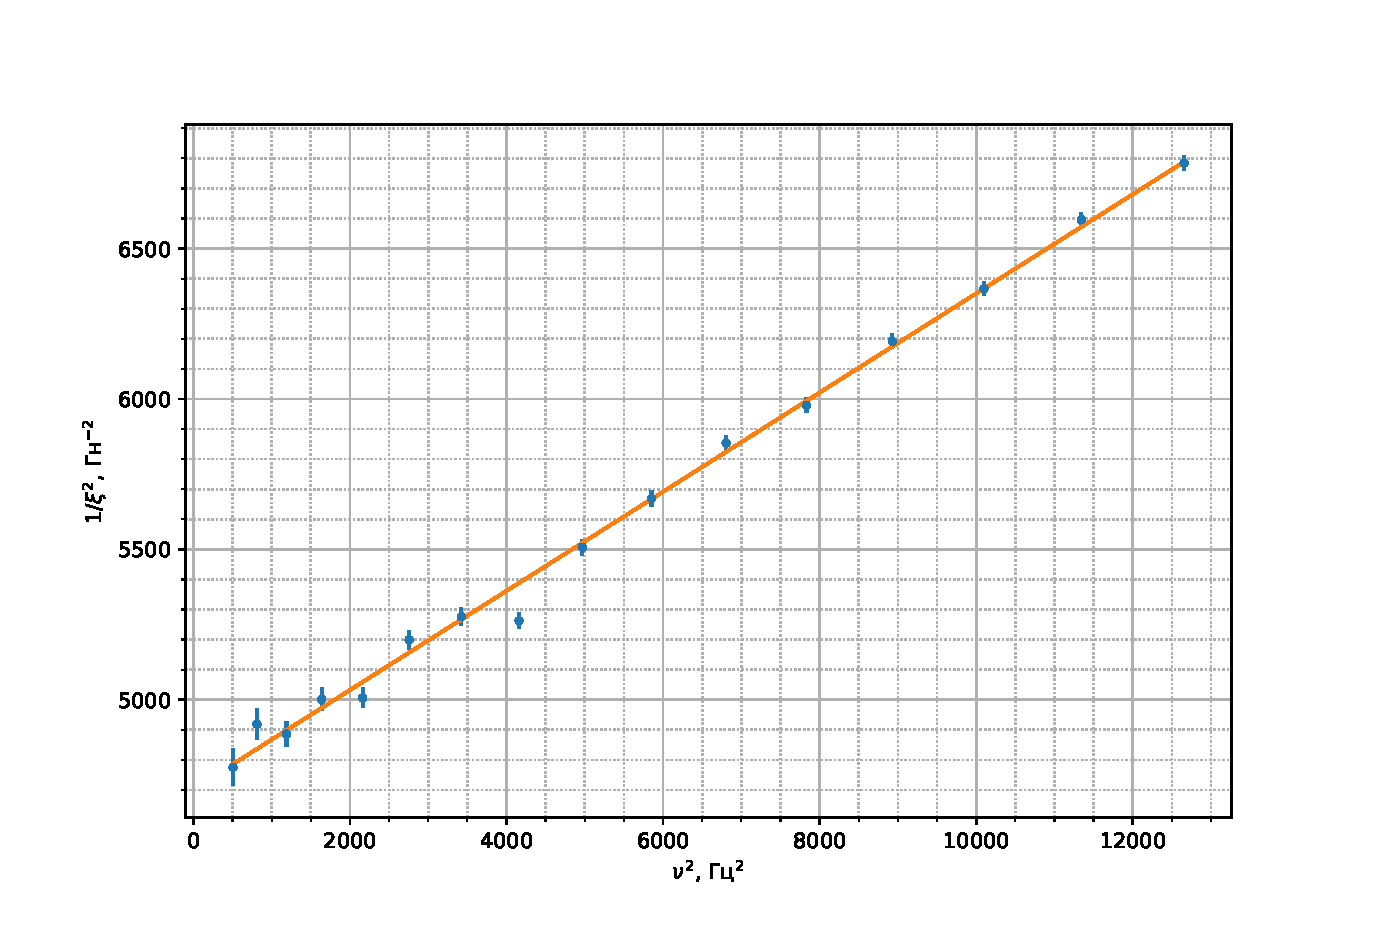
\includegraphics[width=\linewidth]{ksi1.eps}
\end{figure}

Получаем значения линейной зависимости $y=k_1x+1/\xi_0^2$

$k_1=0.16\frac{1}{Гн^2Гц^2}$ $\varepsilon_{k_1}=0.01$

$\xi_0=0.0145 Гн$ $\varepsilon_{\xi_0}=0.01$

Далее построим зависимость $\sqrt{\frac{|H_1|}{|H_0|}^2-1}(\nu)$ Эта зависимость будет также являться линейной.

\begin{figure}[H]
    \centering
    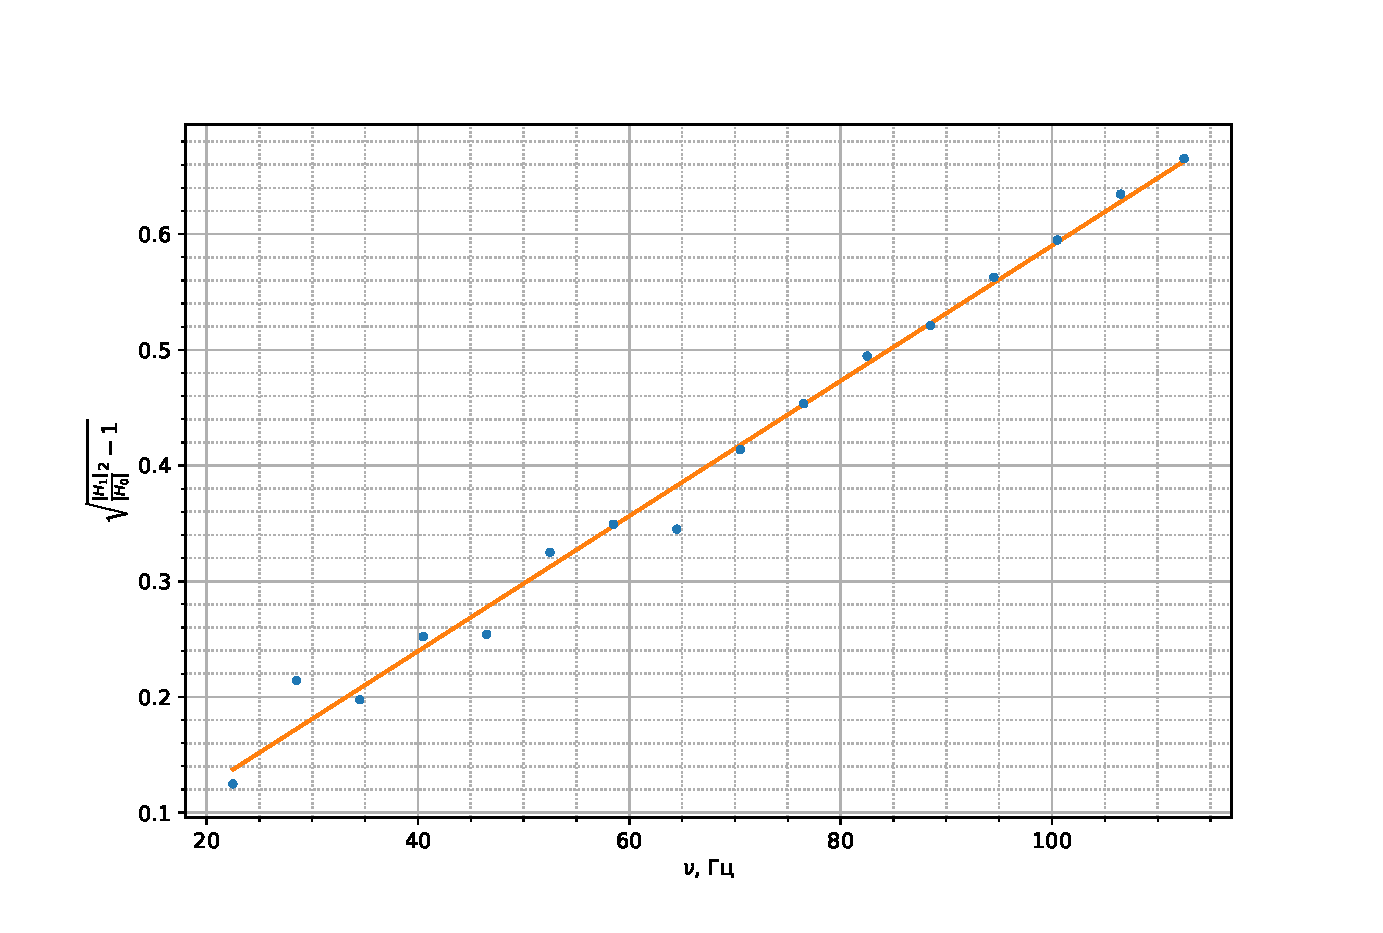
\includegraphics[width=\linewidth]{sigm.eps}
\end{figure}

получаем угловой коэффициент $k_2=5.8\cdot10^{-3}\frac{1}{Гн}$ $\varepsilon_{k_2}=0.025$ 

Отсюда находим через формулу $\sigma=\frac{k_2}{\pi\mu_0ah}$, $\sigma=4.4$ МСименс/м, $\varepsilon_{\sigma}=0.025$.

Теперь построим зависимость для малых частот. Из теории линейным должно быть $\tan{\psi}(\nu)$

\begin{figure}[H]
    \centering
    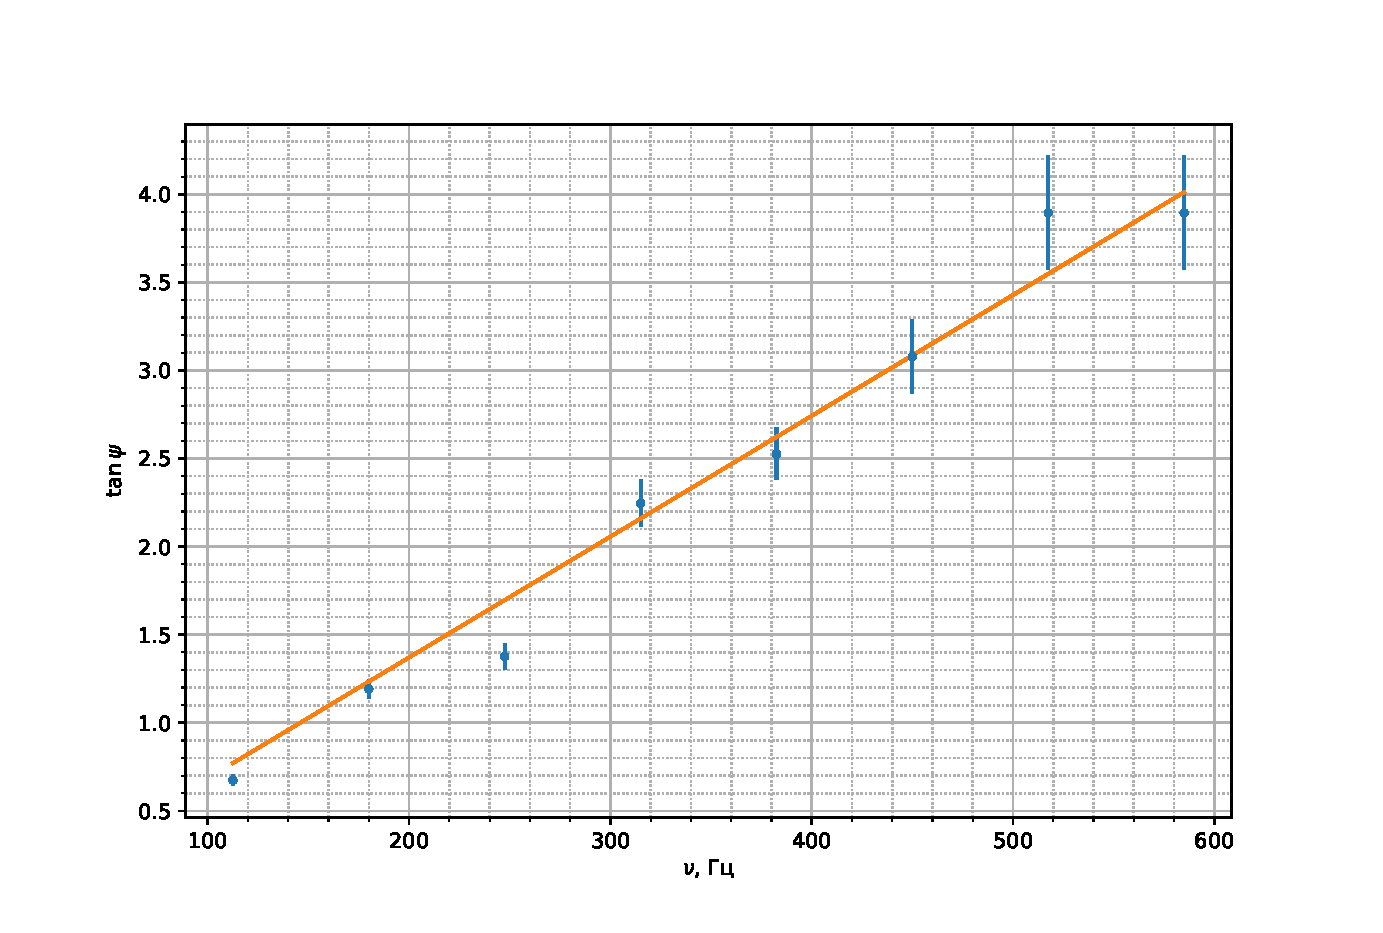
\includegraphics[width=\linewidth]{izm1.eps}
\end{figure}

Аппроксимируем прямой через 0. Получаем $k_3=7.3\cdot10^{-3}\frac{1}{Гн}$ $\varepsilon_{k_3}=0.026$ и из этого вычисляем по формуле $\sigma=\frac{k_3}{\pi\mu_0ah}$, $\sigma=5.1$ МСименс/м,  $\varepsilon_{\sigma}=0.026$.

И теперь при высоких частотах. Из теории построим 
\begin{figure}[H]
    \centering
    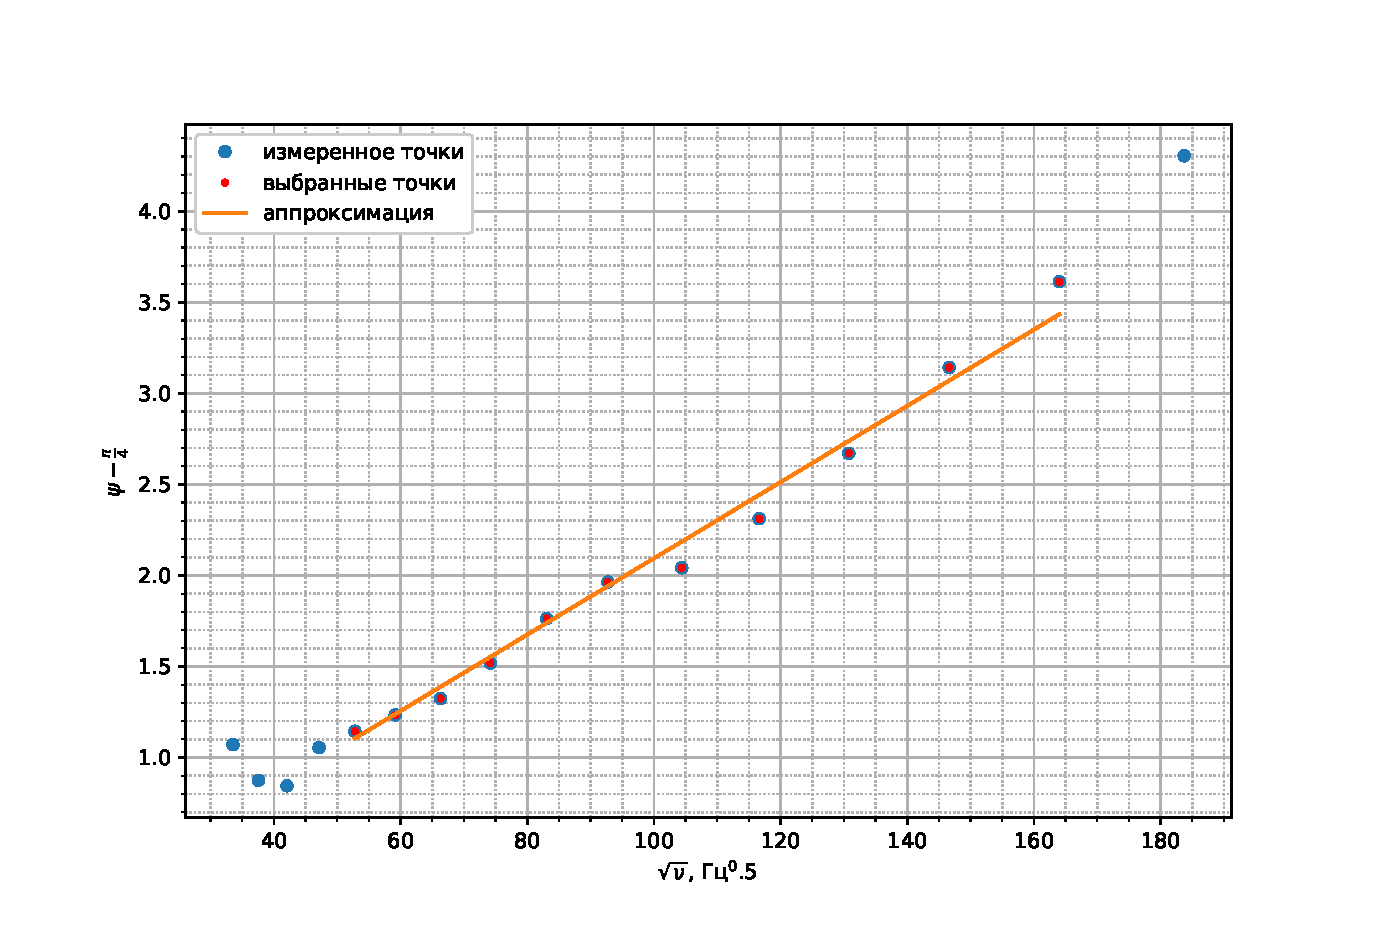
\includegraphics[width=\linewidth]{izm2.eps}
\end{figure}

Аналогично используем прямую через 0. Получаем $k_4=2.1\cdot10^{-2}\frac{1}{Гн}$ и из этого вычисляем по формуле $\sigma=\frac{k_4^2}{\pi\mu_0h^2}$, $\sigma=4.9$ МСименс/м, $\varepsilon_{\sigma}=0.01$.

И теперь по этим данным сравним значения отношения $\frac{|H_1|}{|H_0|}$ при разных $\sigma$.

\begin{figure}[H]
    \centering
    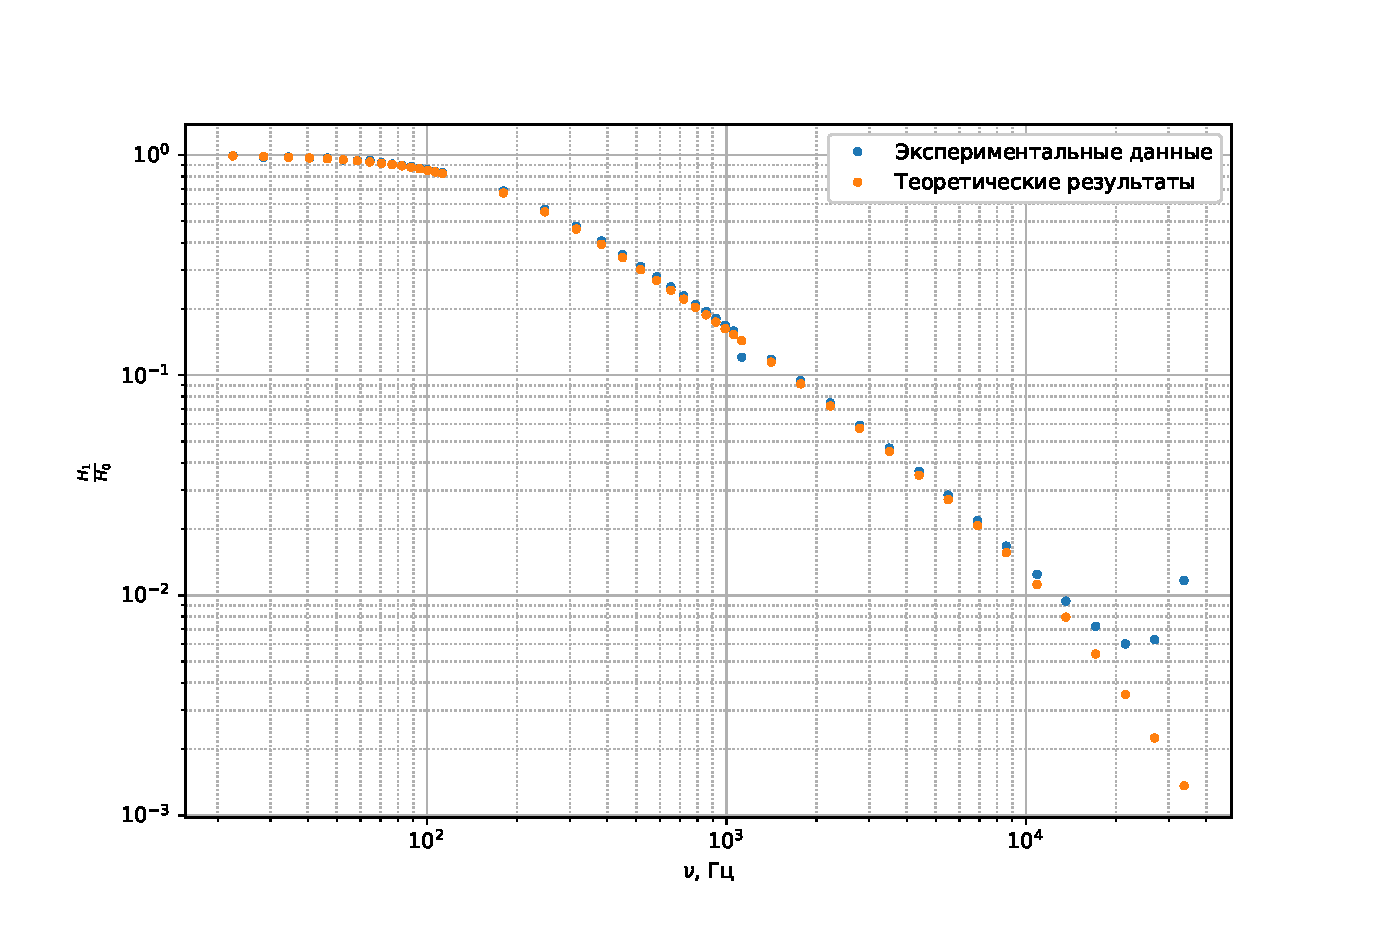
\includegraphics[width=\linewidth]{h1h0.eps}
    \caption{Графики для $\sigma=4.4$ МСименс/м}
\end{figure}

\begin{figure}[H]
    \centering
    \includegraphics[width=\linewidth]{h1h02.eps}
    \caption{Графики для $\sigma=4.9$ МСименс/м}
\end{figure}

Теория начинает расходится на высоких частотах.

\section{ Обсуждение результатов и выводы}
В итоге мы подтвердили существование скин-эффекта и получили проводимость меди в исследуемом оборудовании. Также видно, что приближения нашей теории неверны при слишком больших частотах.

В ходе выполнения возникла проблема точного измерения сдвига.


\end{document}
